\section{Modellkoordinatensystem}\label{kap:model_coordinate_system}

Bei der Aufnahme des Spielstandes über eine Kamera können die Kugeln im Bild erkannt und deren Zentrum, was der
Position entspricht, in Pixelkoordinaten im Bild ermittelt werden.
Die Pixelkoordinaten sind für die weitere Verarbeitung, sei es Analyse und Darstellung des Spielstandes oder Simulation
von Spielzügen, nicht geeignet. Es wird ein Koordinatensystem benötigt, welches möglichst unabhängig von der Auflösung,
Position und Blickrichtung der Kamera ist.

Idealerweise werden die Pixelkoordinaten in ein zu definierendes Koordinatensystem transformiert, welches für die weitere
Verarbeitung verwendet werden kann. Nachfolgend wird dieses Koordinatensystem, das Modellkoordinatensystem genannt wird,
und wie folgt definiert ist:
\begin{enumerate}
  \item Das Koordinatensystem ist zweidimensional.
  \item Der Ursprung befindet sich in der Mitte des Billiardtisches auf Höhe der Kugelmittelpunkte.
  \item Die X-Achse ist parallel zu der längeren Seite und die Y-Achse ist parallel zu der kürzeren Seite des Tisches.
  \item Die Länge eines Einheitsvektors entspricht 1\si{\milli\metre}.
\end{enumerate}

Diese Definition ist insofern praktisch, als dass die Banden und Löcher des Billiardtischs sehr einfach in diesem
Koordinatensystem definiert werden können.
In Abbildung \ref{fig:table_model_coordinate_system} ist der Ursprung und die Achsen des Koordinatensystems eingezeichnet.

\begin{figure}[h!]
    \begin{center}
    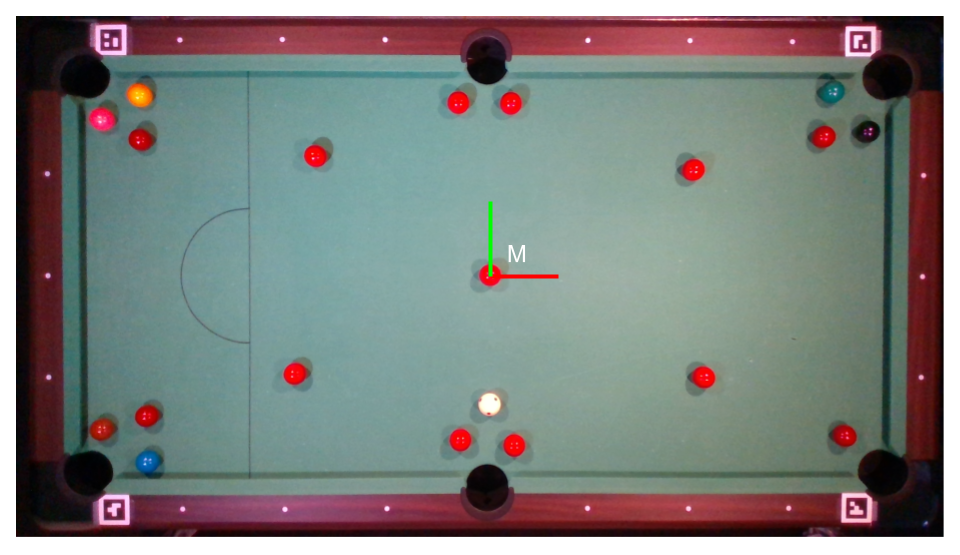
\includegraphics[width=0.8\linewidth]{../common/resources/coordinate_systems/table_model_coordinate_system.png}
    \end{center}
    \caption{Modellkoordinatensystem}
    \label{fig:table_model_coordinate_system}
\end{figure}

Die Transformation vom Pixelkoordinatensystem zum Modellkoordinatensystem erfolgt über mehrere Koordinatensystemtransformationen:
\begin{enumerate}
  \item \label{item:transforms_pixel_to_camera} Pixelkoordinaten zu Kamerakoordinaten, siehe Abschnitt \ref{kap:pixel_to_camera}
  \item \label{item:transforms_camera_to_world} Kamerakoordinaten zu Weltkoordinaten, siehe Abschnitt \ref{kap:camera_to_world}
  \item \label{item:transforms_world_to_rail} Weltkoordinaten zu Bandenkoordinaten, siehe Abschnitt \ref{kap:world_to_rail}
  \item \label{item:transforms_rail_to_model} Bandenkoordinaten zu Modellkoordinaten, siehe Abschnitt \ref{kap:rail_to_model}
\end{enumerate}

Alle Koordinatensysteme bis auf das Pixelkoordinatensystem sind in der Einheit Millimeter definiert,
um nicht benötigte Skalierungen in den Transformationen zu vermeiden.


\subsection{Pixelkoordinaten zu Kamerakoordinaten}\label{kap:pixel_to_camera}

Für die Transformation von Pixelkoordinaten zu Kamerakoordinaten wird die intrinsische Kameramatrix und
die Grösse der Sensorpixel der verwendeten Kamera benötigt.
Die intrinsische Kameramatrix $K$ ist nachfolgend erneut aufgeführt, diese wurde zusammen mit der
verwendeten Kamera in Abschnitt \ref{kap:camera} beschrieben.

\begin{align}
K =
\begin{pmatrix}
    f_x & s   & c_x\\
    0   & f_y & c_y\\
    0   & 0   & 1
\end{pmatrix}
\end{align}

Nun soll ein 2D-Punkt im Pixelkoordinatensystem in einen 3D-Punkt im Kamerakoordinatensystem überführt werden.
Sei der Pixelpunkt $p = (p_x, p_y)$, dann kann diesem der \emph{principal point} $c = (c_x, c_y)$ abgezogen werden, um den Ursprung in
die Mitte des Bildsensors zu verschieben. Anschliessend müssen die Koordinaten mit der
Sensorgrösse $s = (s_x, s_y)$ [\si{\milli\metre}] skaliert werden, um die Koordinaten von der Einheit Pixel
in die Einheit Millimeter umzuwandeln. Die Z-Komponente des resultierenden Punktes $P_C$ im Kamerakoordinatensystem ist
die Brennweite aus der intrinsischen Kameramatrix. Dabei gilt es zu beachten, dass die Parameter $f_x$ und $f_y$ der
intrinsischen Kameramatrix in der Einheit Pixel sind, und daher ebenfalls mit der Sensorgrösse $s$ skaliert werden müssen.

\begin{align}
f = f_x \cdot s_x\\
P_{C,x} = (p_x - c_x) \cdot s_x\\
P_{C,y} = (p_y - c_y) \cdot s_y\\
P_{C,z} = f\\
P_C = \begin{pmatrix}P_{C,x}\\P_{C,y}\\P_{C,z}\end{pmatrix}
\end{align}

% TODO: evtl. Bild einfügen (dieses wäre gut: https://learnopencv.com/geometry-of-image-formation/)

Damit ist diese Transformation abgeschlossen und der Punkt in Kamerakoordinaten kann in Weltkoordianten übersetzt werden.

\subsection{Kamerakoordinaten zu Weltkoordinaten}\label{kap:camera_to_world}

Der Punkt $P_C$ in Kamerakoordinaten muss nun in die reale Welt überführt werden. Da der Punkt $P_C$ relativ zur Kamera
positioniert ist, muss die Position der Kamera in der realen Welt bestimmt werden.
Somit braucht es eine \emph{pose estimation} der Kamera, d.H. die Position und Orientierung der Kamera in der realen Welt müssen bestimmt werden.
Eine \emph{pose estimation} benötigt eine kalibrierte Kamera und ein Objekt bekannter Grösse, welches im Bild erkannt werden kann.

Als Objekt bekannter Grösse und Position wurde ein ArUco-Board \cite{opencv:detection_of_aruco_boards} mit vier Markern verwendet.
Die verwendeten Marker mit einer Seitenlänge von 50\si{\milli\metre} und einer Grösse von 3x3 bits sind
in Abbildung \ref{fig:used_aruco_markers} aufgeführt.

\begin{figure}[h!]
    
\includegraphics[width=0.2\linewidth]{../common/resources/aruco/marker_0.png}
    
\includegraphics[width=0.2\linewidth]{../common/resources/aruco/marker_1.png}
    
\includegraphics[width=0.2\linewidth]{../common/resources/aruco/marker_2.png}
    
\includegraphics[width=0.2\linewidth]{../common/resources/aruco/marker_3.png}
    \caption{Verwendete ArUco markers}
    \label{fig:used_aruco_markers}
\end{figure}

Diese Marker wurden auf dem Tisch wie in Abbildung \ref{fig:table_with_aruco_markers} angebracht und deren relative
Position zueinander ausgemessen.

\begin{figure}[h!]
    \begin{center}
    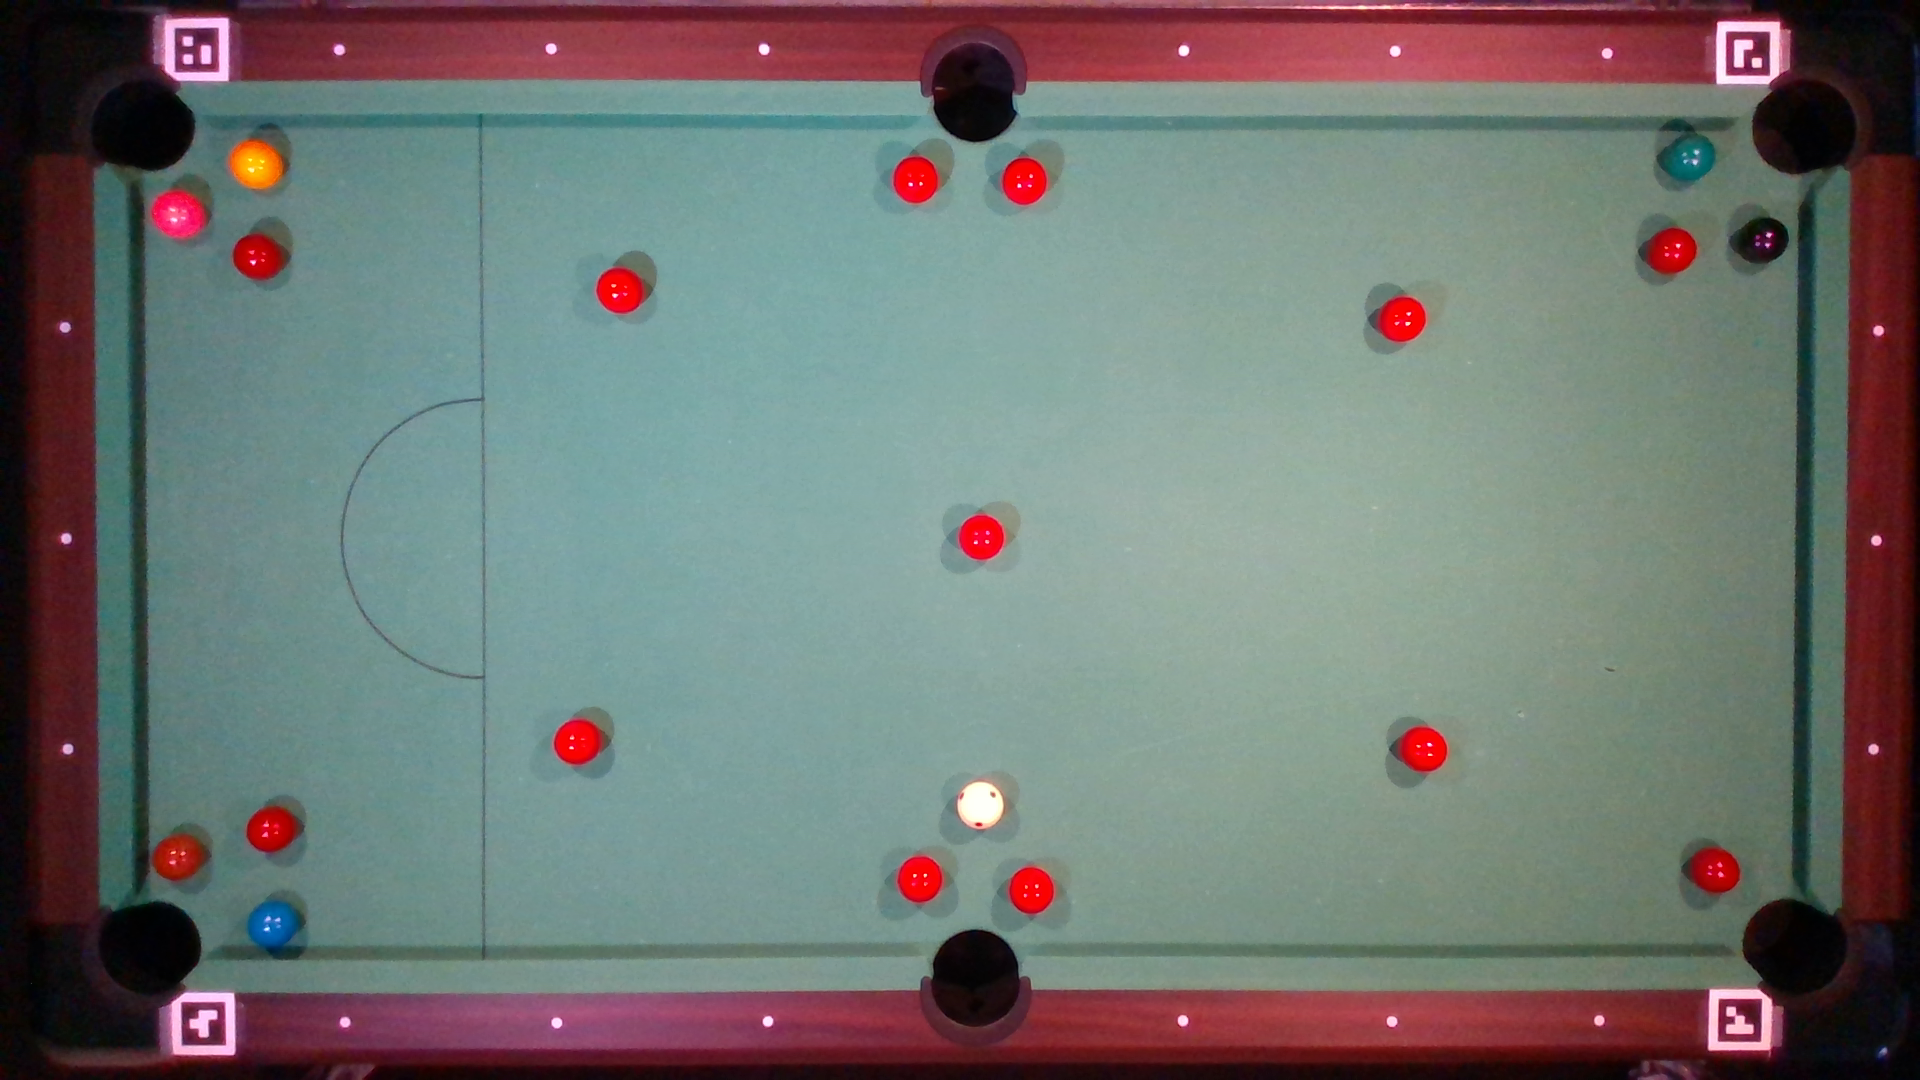
\includegraphics[width=0.6\linewidth]{../common/resources/coordinate_systems/table_with_markers.png}
    \end{center}
    \caption{Billiardtisch mit ArUco markers}
    \label{fig:table_with_aruco_markers}
\end{figure}

Das ArUco board ist definiert, sobald alle Eckpunkte der einzelnen Marker relativ zu einem
gewählten Weltkoordinatenursprung bekannt sind. Als Ursprung wurde der Mittelpunkt des Markers
in Abbildung \ref{fig:table_world_coordinate_system} unten links gewählt.
Die X-Achse ist parallel zur langen Seite des Tischs und die Y-Achse ist parallel zur kurzen Seite des Tischs.

\begin{figure}[h!]
    \begin{center}
    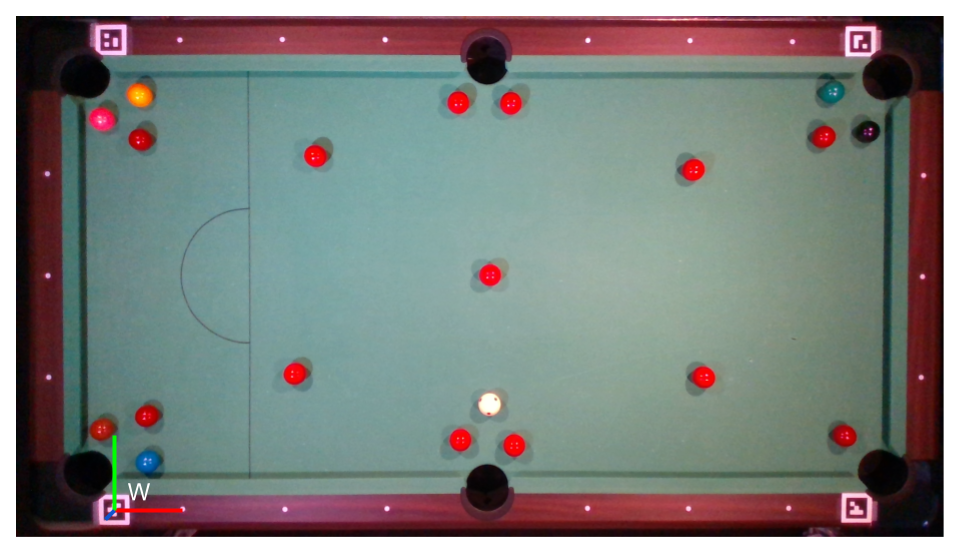
\includegraphics[width=0.6\linewidth]{../common/resources/coordinate_systems/table_world_coordinate_system.png}
    \end{center}
    \caption{Weltkoordinatensystem}
    \label{fig:table_world_coordinate_system}
\end{figure}

Mit der Definition des bekannten Objekts in der realen Welt kann nun die \emph{pose estimation} durchgeführt werden,
um daraus die extrinsische Kameramatrix zu bestimmen. Die extrinsische Kameramatrix $E$ beschreibt die Transformation eines
Punkts $P_W$ in Weltkoordinaten zu einem Punkt $P_C$ in Kamerakoordinaten und ist wie folgt definiert \cite{simek:extrinsic_camera_matrix}:

\begin{align}
E =
\begin{pmatrix}
    r_{1,1} & r_{1,2} & r_{1,3} & t_1\\
    r_{2,1} & r_{2,2} & r_{2,3} & t_2\\
    r_{3,1} & r_{3,2} & r_{3,3} & t_3\\
    0       & 0       & 0       & 1
\end{pmatrix}
\end{align}

Die inverse Transformation $E^{-1}$ transformiert einen Punkt $P_C$ in Kamerakoordinaten in einen Punkt $P_W$ in Weltkoordinaten.
So kann die Position der Kamera in Weltkoordinaten $C_W$ anhand der Position in Kamerakoordinaten $C_C$ und der Matrix $E^{-1}$ bestimmt werden:
\begin{align}
C_C = \begin{pmatrix} 0 \\ 0 \\ 0 \\ 1 \end{pmatrix}\\
C_W = E^{-1} \cdot C_C
\end{align}

Ebenso kann die Position des Pixels in Weltkoordianten $P_W$ bestimmt werden, wobei $P_C$
in Abschnitt \ref{kap:pixel_to_camera} erarbeitet wurde:

\begin{align}
P_C = \begin{pmatrix}P_{C,x}\\P_{C,y}\\P_{C,z}\end{pmatrix}\\
P_W = E^{-1} \cdot P_C
\end{align}

Es gilt zu beachten, dass die Position des Pixels in Weltkoordinaten $P_W$ nicht der Position der Kugel, welche evtl. an
dieser Pixelposition detektiert wurde, entspricht. Die projektive Abbildung der realen Welt auf den Bildsensor kann
nicht rückgängig gemacht werden, weil die Tiefeninformation verloren gegangen ist.

Da bekannt ist, dass sich alle Mittelpunkte der Kugeln auf dem Tisch auf einer Ebene befinden, kann die Pixelkoordinate
eines Kugelmittelpunkts trotzdem in eine Weltkoordinate transformiert werden.
Es gilt die Weltkoordinate $B_W$ der Kugel zu bestimmen.
Dazu kann eine Linie $L$ zwischen Kamera-Weltkoordinate $C_W$ und Pixel-Weltkoordinate $P_W$ gezogen werden und deren
Schnittpunkt mit der Ebene $\Sigma$, welche auf Höhe der Kugelmittelpunkte in Weltkoordinaten $H$ ist, bestimmt werden.
Die Linie $L$ ist in der Parameterform mit dem Stützvektor $\vec{q}$ und dem Richtungsvektor $\vec{v}$ und dem Skalierungsfaktor $\lambda$ definiert.
Sei $B$ eine Ebene in der Normalenform mit dem Stützvektor $\vec{a}$ und dem Normalenvektor $\vec{n}$, dann gilt:

\begin{align}
C_W = E^{-1} \cdot C_C\\
P_W = E^{-1} \cdot P_C\\
\vec{q} = C_W\\
\vec{v} = P_W - C_W\\
L: \vec{B_W} = \vec{q} + \lambda \cdot \vec{v}\\
\vec{a} = \begin{pmatrix}0\\0\\H\end{pmatrix}\\
\vec{n} = \begin{pmatrix}0\\0\\1\end{pmatrix}\\
\Sigma: (\vec{B_W} - \vec{a}) \cdot \vec{n} = 0\\
\end{align}

Durch Einsetzen der Liniengleichung in die Ebenengleichung kann der Schnittpunkt ermittelt werden.

\begin{align}
(\vec{q} + \lambda \cdot \vec{v} - \vec{a}) \cdot \vec{n} = 0\\
\vec{q} \cdot \vec{n} + \lambda \cdot \vec{v} \cdot \vec{n} - \vec{a} \cdot \vec{n} = 0\\
\lambda \cdot \vec{v} \cdot \vec{n} = \vec{a} \cdot \vec{n} - \vec{q} \cdot \vec{n}\\
\lambda \cdot \vec{v} \cdot \vec{n} = (\vec{a} - \vec{q}) \cdot \vec{n}\\
\lambda = \frac{(\vec{a} - \vec{q}) \cdot \vec{n}}{\vec{v} \cdot \vec{n}}
\end{align}

Falls $\vec{v} \cdot \vec{n} = 0$ gilt, dann gibt es keinen Schnittpunkt.
Die Kugel-Weltkoordinate kann durch Skalierung der Linie bestimmt werden:

\begin{align}
B_W = \vec{q} + \lambda \cdot \vec{v}\\
B_W = C_W + \lambda \cdot (P_W - C_W)\\
B_W = C_W + \frac{(\vec{a} - \vec{q}) \cdot \vec{n}}{\vec{v} \cdot \vec{n}} \cdot (P_W - C_W)
\end{align}

Damit ist die Weltkoordinate des Kugelmittelpunkts $B_W$ anhand dessen Pixel-Weltkoordinate $P_W$ ermittelt.


\subsection{Weltkoordinaten zu Bandenkoordinaten}\label{kap:world_to_rail}

Die vorletzte Transformation von Weltkoordinaten zu Bandenkoordinaten ist eine einfache Translation des Ursprungs,
siehe dazu Abbildung \ref{fig:table_world_to_rail}. Der Ursprung wird nicht rotiert, lediglich verschoben.
Diese Verschiebung kann auch in der Angabe der Weltkoordinaten des ArUco boards berücksichtigt werden, wodurch diese
Translation obsolet wird. Sie wurde belassen, da dies eine kleine Operation darstellt und dadurch das Ausmessen des
ArUco boards und dessen Verschiebung zum Bandenursprung klar getrennt ist.

\begin{figure}[h!]
    \begin{center}
    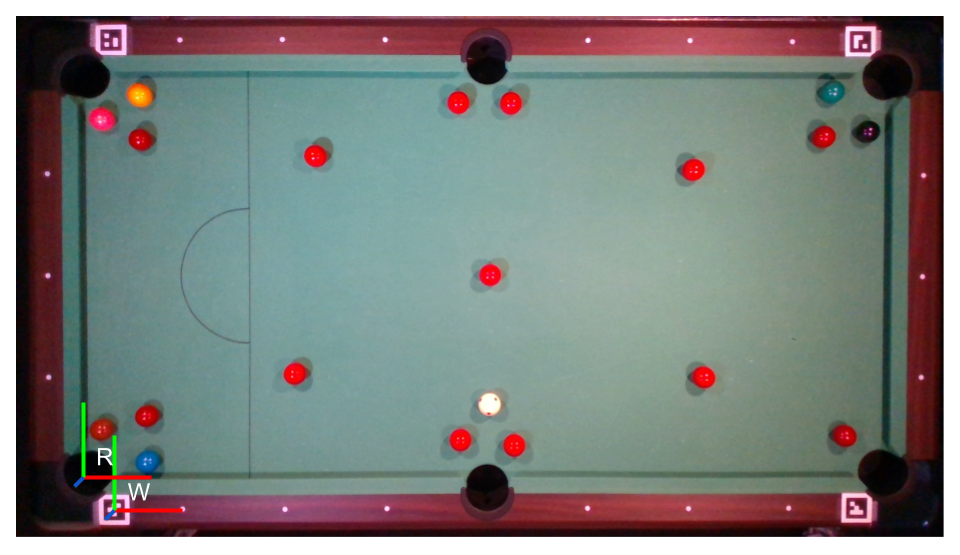
\includegraphics[width=0.6\linewidth]{../common/resources/coordinate_systems/table_world_to_rail.png}
    \end{center}
    \caption{Welt-Ursprung W und Banden-Ursprung R}
    \label{fig:table_world_to_rail}
\end{figure}


Wenn die Verschiebung von Welt-Ursprung zu Banden-Ursprung $T_{wb} = (\Delta x, \Delta y)$, dann ist
die Kugelposition in Bandenkoordinaten $B_R$:

\begin{align}
B_R = B_W + \begin{pmatrix}\Delta x\\\Delta y\\0\end{pmatrix}
\end{align}

Somit steht nur noch die letzte Transformation bevor.


\subsection{Bandenkoordinaten zu Modellkoordinaten}\label{kap:rail_to_model}

Zuletzt wird der Ursprung erneut verschoben, vom Ursprung des Bandenkoordinatensystems zum
Ursprung des Modellkoordinatensystems, siehe dazu Abbildung \ref{fig:table_rail_to_model}.

\begin{figure}[h!]
    \begin{center}
    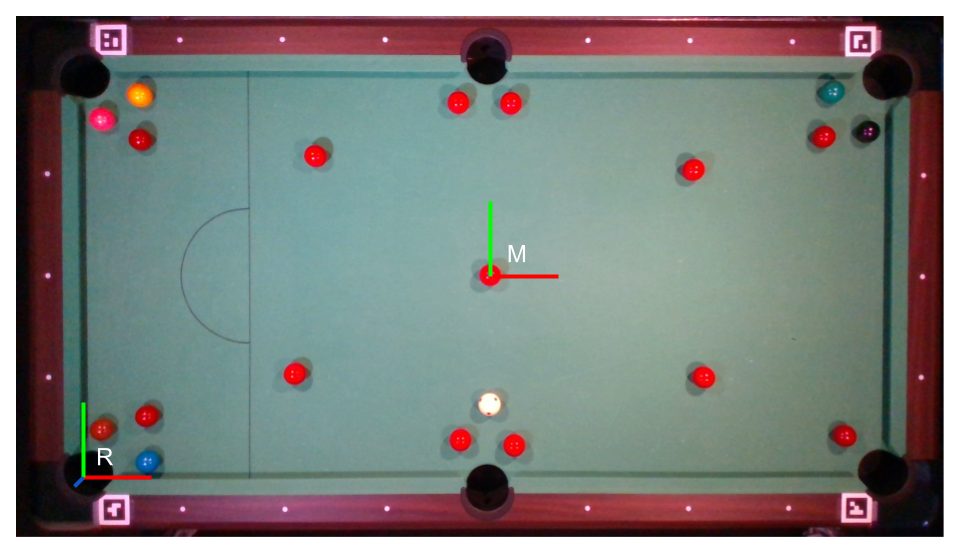
\includegraphics[width=0.6\linewidth]{../common/resources/coordinate_systems/table_rail_to_model.png}
    \end{center}
    \caption{Banden-Ursprung B und Modell-Ursprung R}
    \label{fig:table_rail_to_model}
\end{figure}

Für diese Verschiebung muss lediglich die Länge und Breite des Bereichs, welcher von den Banden begrenzt wird,
gemessen werden, siehe Abbildung \ref{fig:table_inner_lengths}.

\begin{figure}[h!]
    \begin{center}
    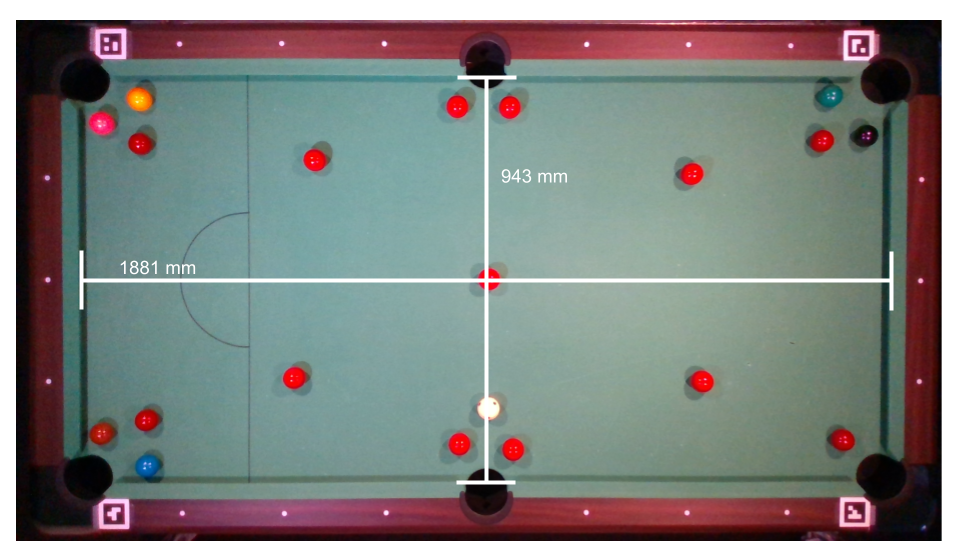
\includegraphics[width=0.6\linewidth]{../common/resources/coordinate_systems/table_inner_lengths.png}
    \end{center}
    \caption{Länge und Breite des Spielbereits}
    \label{fig:table_inner_lengths}
\end{figure}

Wenn der Spielbereich die Länge $L$ und Breite $B$ hat, dann ist die Kugelposition in Modellkoordinaten $B_M$:

\begin{align}
\Delta x = \frac{L}{2}\\
\Delta y = \frac{B}{2}\\
B_M = B_R - \begin{pmatrix}\Delta x\\\Delta y\\0\end{pmatrix}
\end{align}

Somit konnte die Kugelposition in Pixelkoordinaten in ein Modellkoordinatensystem umgewandelt werden, welches für
die weitere Verarbeitung von Nutzen ist.
